% reports/talk.tex
% Compile: pdflatex reports/talk.tex   (run twice for frame numbers)
% Requires lstlean.tex installed globally (already on this machine).
\documentclass[10pt,aspectratio=169]{beamer}

\usepackage[T1]{fontenc}
\usepackage[utf8]{inputenc}
\usepackage{amssymb}
\usepackage{upgreek}
\usepackage{color}

% lstlean.tex expects these named colors to be defined.
\definecolor{keywordcolor}{rgb}{0.7, 0.1, 0.1}
\definecolor{tacticcolor}{rgb}{0.0, 0.1, 0.6}
\definecolor{commentcolor}{rgb}{0.4, 0.4, 0.4}
\definecolor{symbolcolor}{rgb}{0.0, 0.1, 0.6}
\definecolor{sortcolor}{rgb}{0.1, 0.5, 0.1}
\definecolor{attributecolor}{rgb}{0.7, 0.1, 0.1}
\definecolor{errorcolor}{rgb}{1, 0, 0}
\definecolor{stringcolor}{rgb}{0.5, 0.3, 0.2}

\usepackage{listings}
\def\lstlanguagefiles{lstlean.tex}
\lstset{language=lean}

\usepackage{tikz}
\usetikzlibrary{arrows.meta, positioning, calc, fit, backgrounds}

% ---- minimal beamer styling -------------------------------------------------
\usetheme{default}
\setbeamertemplate{navigation symbols}{}
\setbeamertemplate{footline}[frame number]
\setbeamerfont{frametitle}{size=\large,series=\bfseries}
\setbeamercolor{frametitle}{fg=black}
\setbeamercolor{structure}{fg=black!75}
\setbeamertemplate{itemize item}{\textbullet}

\hypersetup{colorlinks=true, urlcolor=blue!60!black, linkcolor=blue!60!black}

% ---- listings: tighten layout for slides (keep language=lean from preamble) -
\lstset{
  basicstyle=\ttfamily\scriptsize,
  keywordstyle=\bfseries,
  commentstyle=\itshape\color{black!55},
  showstringspaces=false,
  columns=fullflexible,
  breaklines=true,
  xleftmargin=4pt,
  aboveskip=4pt, belowskip=4pt,
}

% ---- shared TikZ styles -----------------------------------------------------
\tikzset{
  box/.style    ={draw, rounded corners=2pt, align=center,
                  minimum height=0.95cm, minimum width=2.6cm, font=\small},
  pill/.style   ={draw, dashed, rounded corners=2pt, align=center,
                  minimum height=0.7cm, font=\scriptsize, inner sep=3pt},
  arr/.style    ={-{Stealth[length=2.2mm]}, thick},
  lbl/.style    ={font=\scriptsize, inner sep=1pt},
}

\title{Who sacked my cluster?}
\author{Sachin Singh}
\date{}

\begin{document}

% ---------------------------------------------------------------------------
\begin{frame}
  \titlepage
  \vspace{-1.0em}
  \centerline{\small\url{https://github.com/sachinkumarsingh092/lean-rl/tree/master/lean_rl/lean}}
\end{frame}

% ---------------------------------------------------------------------------
\begin{frame}{The problem}
\begin{itemize}\itemsep0.4em
  \item LLM-driven SRE agents propose operations on a \hyperlink{glossary}{Kubernetes} cluster.
  \item The agent is non-deterministic; we cannot trust it to be safe.
  \item \textbf{Idea:} between ``agent emits action'' and ``cluster executes action'',
        there is a \emph{Lean-checked admission gate} that accept a machine-checkable
        proof and gives a structured reason output that becomes RL feedback.
\end{itemize}
\vspace{0.6em}
\begin{center}
\itshape I've made a SFT + RL gym as a use-case for this which I used to train a small model. But I've only explained the Lean side here.
\end{center}
\end{frame}

% ---------------------------------------------------------------------------
\begin{frame}{Architecture}
\centering
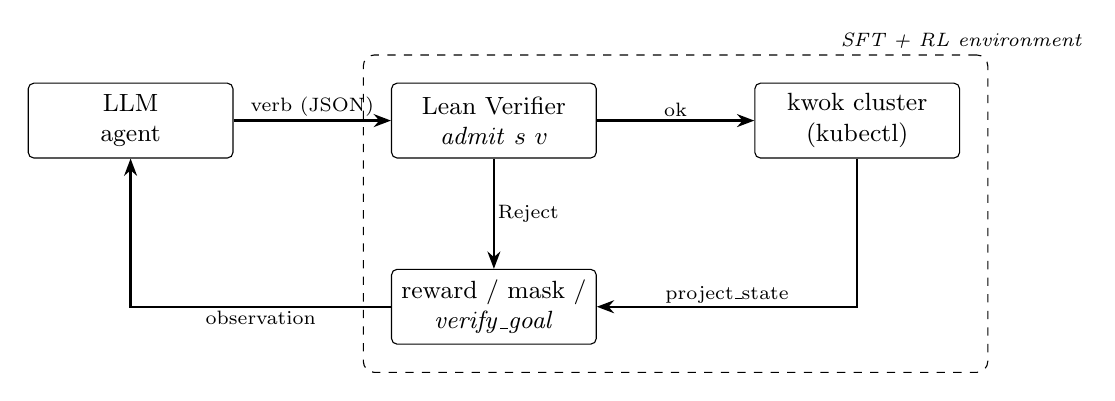
\begin{tikzpicture}[node distance=1.6cm and 2.0cm]
  \node[box]                       (llm)  {LLM\\agent};
  \node[box, right=of llm]         (lean) {Lean Verifier\\$\mathit{admit}\ s\ v$};
  \node[box, right=of lean]        (kwok) {kwok cluster\\(kubectl)};
  \node[box, below=1.4cm of lean]  (rwd)  {reward / mask /\\$\mathit{verify\_goal}$};

  \draw[arr] (llm)  -- node[lbl, above]{verb (JSON)} (lean);
  \draw[arr] (lean) -- node[lbl, above]{ok}          (kwok);
  \draw[arr] (lean) -- node[lbl, right]{Reject}      (rwd);
  \draw[arr] (kwok) |- node[lbl, pos=0.75, above]{project\_state} (rwd);
  \draw[arr] (rwd)  -| node[lbl, pos=0.25, below]{observation}    (llm);

  \begin{scope}[on background layer]
    \node[draw, dashed, rounded corners=4pt, inner sep=10pt,
          fit=(lean)(kwok)(rwd),
          label={[font=\scriptsize\itshape, inner sep=2pt]
                  above right:SFT + RL environment}]
          (envbox) {};
  \end{scope}
\end{tikzpicture}
\vspace{0.6em}
\centerline{\small Lean = judge \quad\textbar\quad kwok = world (source of truth)}
\end{frame}

% ---------------------------------------------------------------------------
\begin{frame}{A small Kubernetes glossary}\label{glossary}
\scriptsize
\begin{columns}[T,onlytextwidth]
\begin{column}{0.48\textwidth}
\begin{description}\itemsep0.25em
  \item[Kubernetes] Open-source orchestration system for containerized workloads. Provides a declarative API for cluster objects and controllers that drive actual state toward desired state.
  \item[Pod] One or more containers running together as a unit. Modeled as a \texttt{Pod} struct with \texttt{phase}, \texttt{node}, and a resource \texttt{request}.
  \item[Node] A worker machine that hosts pods. Has a \texttt{capacity} (CPU and memory) and a \texttt{cordoned} flag.
  \item[Deployment] Desired-state spec saying ``I want N replicas of this image''. The control loop tries to keep that count.
  \item[Replica] One running pod belonging to a deployment. \texttt{availableReplicas} counts the Running ones.
  \item[Capacity] The sum of all pod requests on a node must not exceed the node's CPU and memory capacity.
  \item[kwok] A project that simulates the Kubernetes API, so we can act on a cluster without running real workloads (\href{https://kwok.sigs.k8s.io/}{kwok.sigs.k8s.io}).
\end{description}
\end{column}
\begin{column}{0.48\textwidth}
\begin{description}\itemsep0.25em
  \item[PDB] Pod Disruption Budget. A per-deployment promise that at least \texttt{minAvailable} replicas stay Running across voluntary disruptions.
  \item[Anti-affinity] Scheduling rule: no two pods of the same deployment land on the same node.
  \item[resourceVersion] Opaque counter that bumps on every change. The agent echoes the version it last saw, so concurrent edits cannot silently overwrite.
  \item[Admission webhook] Real Kubernetes extension point where the API server calls out before persisting an object. Our \texttt{admit} is a Lean-checked admission webhook.
  \item[Drain / cordon] Mark a node unschedulable, then evict its pods.
  \item[kubectl] The Kubernetes command-line client. We use it to push admitted verbs to kwok.
\end{description}
\end{column}
\end{columns}
\end{frame}

% ---------------------------------------------------------------------------
\begin{frame}[fragile]{The Lean stack}
\begin{lstlisting}
import ProvedSRE.Cluster      -- ADTs: Pod, Node, Deployment, State; step
import ProvedSRE.Invariants   -- pdbRespected, capacityRespected, antiAffinityRespected, safe
import ProvedSRE.Api          -- ApiVerb, apply, preCheck, postCheck, admit
import ProvedSRE.Goals        -- episode termination predicates
import ProvedSRE.Soundness    -- theorem admitSafe : admit s v = .ok () -> safe (apply s v)
import ProvedSRE.Verify       -- FromJson/ToJson + stdin/stdout JSON line server
\end{lstlisting}
\vspace{0.4em}
\textbf{Toolchain:} \texttt{leanprover/lean4:v4.29.0}, \emph{no} mathlib (pure core Lean 4).
\end{frame}

% ---------------------------------------------------------------------------
\begin{frame}[fragile]{Decidable invariants}
\begin{lstlisting}
def pdbRespected (s : State) : Bool :=
  s.deployments.all fun d => availableReplicas s d.id ≥ d.minAvailable

inductive InvariantKind | pdb | capacity | antiAffinity

def invariants : List (InvariantKind × (State → Bool)) :=
  [ (.pdb,          pdbRespected),
    (.capacity,     capacityRespected),
    (.antiAffinity, antiAffinityRespected) ]

def safe (s : State) : Bool := invariants.all (·.2 s)
\end{lstlisting}
\vspace{0.4em}
\small Each invariant is a \texttt{Bool} predicate on \texttt{State}. They are registered once in a small table. Adding a new invariant is a single line in that table, and \texttt{safe}, \texttt{postCheck}, and the soundness proof all pick it up automatically.
\end{frame}

% ---------------------------------------------------------------------------
\begin{frame}[fragile]{The admission gate}
\begin{lstlisting}
def postCheck (s' : State) (v : ApiVerb) : Except Reject Unit :=
  invariants.foldlM (init := ()) fun _ ⟨ik, p⟩ =>
    if p s' then .ok ()
    else .error (.forbiddenInvariant ik (verbTarget v) (invariantReason ik))

def admit (s : State) (v : ApiVerb) : Except Reject Unit :=
  match preCheck s v with
  | .error r => .error r
  | .ok _    => postCheck (apply s v) v
\end{lstlisting}
\vspace{0.4em}
\small \texttt{admit} runs the pre-checks first, then dry-runs the verb with \texttt{apply} and re-evaluates every invariant in the registry. This mirrors how a Kubernetes \hyperlink{glossary}{admission webhook} would dry-run an incoming request.
\end{frame}

% ---------------------------------------------------------------------------
\begin{frame}{Inside \texttt{admit}}
\centering
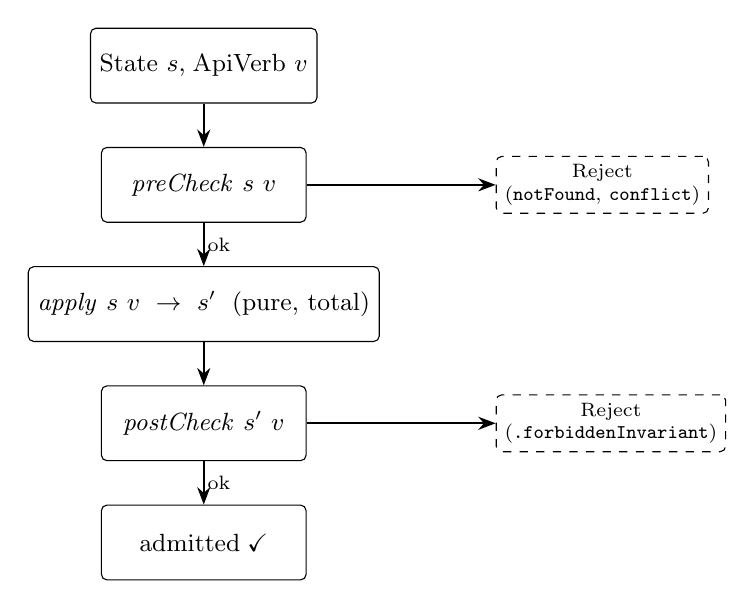
\begin{tikzpicture}[node distance=0.55cm]
  \node[box]                          (in)   {State $s$,\;ApiVerb $v$};
  \node[box, below=of in]             (pre)  {$\mathit{preCheck}\ s\ v$};
  \node[box, below=of pre]            (app)  {$\mathit{apply}\ s\ v\ \to\ s'$ \;(pure, total)};
  \node[box, below=of app]            (post) {$\mathit{postCheck}\ s'\ v$};
  \node[box, below=of post]           (ok)   {admitted\;$\checkmark$};

  \node[pill, right=2.4cm of pre]   (r1) {Reject\\(\texttt{notFound}, \texttt{conflict})};
  \node[pill, right=2.4cm of post]  (r2) {Reject\\(\texttt{.forbiddenInvariant})};

  \draw[arr] (in)   -- (pre);
  \draw[arr] (pre)  -- node[lbl, right]{ok} (app);
  \draw[arr] (app)  -- (post);
  \draw[arr] (post) -- node[lbl, right]{ok} (ok);
  \draw[arr] (pre)  -- (r1);
  \draw[arr] (post) -- (r2);
\end{tikzpicture}
\centerline{\small Everything past this gate is covered by the theorem on the next slide.}
\end{frame}

% ---------------------------------------------------------------------------
\begin{frame}[fragile]{Soundness, completeness, and trace-level safety}
\begin{lstlisting}
theorem postCheck_iff :
    postCheck s' v = .ok () ↔ ∀ p ∈ invariants, p.2 s' = true

theorem admitSafe :
    admit s v = .ok () → safe (apply s v) = true

theorem admit_ok_of_safe :
    preCheck s v = .ok () → safe (apply s v) = true →
    admit s v = .ok ()

theorem runApiPlan_safe :
    safe s = true → runApiPlan s vs = .ok sf → safe sf = true
\end{lstlisting}
\vspace{0.4em}
\small Soundness reduces to a single biconditional that says \texttt{postCheck} accepts a state exactly when every registered invariant holds. The completeness theorem says the gate accepts every plan that is in fact safe. The trace-level theorem lifts safety from a single verb to a full admitted plan by induction.
\end{frame}

% ---------------------------------------------------------------------------
\begin{frame}[fragile]{Episode goals}
\begin{lstlisting}
inductive Goal
  | drainNode    (n : NodeId)
  | rolloutImage (d : DeploymentId) (img : Image)
  | scaleTo      (d : DeploymentId) (replicas : Nat)

def goalAchieved (s : State) : Goal → Bool
  | .drainNode n        =>
      (s.pods.filter fun p => p.node = n ∧ p.phase ≠ .Failed).isEmpty
  | .rolloutImage d img =>
      (s.pods.filter fun p => p.deployment = d ∧ p.phase = .Running).all
        (fun p => p.image = img)
  | .scaleTo d n        => availableReplicas s d = n
\end{lstlisting}
\vspace{0.4em}
\small Goals are typed, decidable predicates on the projected state. After every admitted verb the orchestrator evaluates \texttt{goalAchieved} to decide whether the episode is finished and the goal-completion reward is due.
\end{frame}

% ---------------------------------------------------------------------------
\begin{frame}[fragile]{The wire layer}
\begin{lstlisting}
def handleLine (line : String) : Json :=
  match Json.parse line with
  | .error e => errorResult "" s!"parse: {e}"
  | .ok j    =>
    match (j.getObjValAs? String "mode").toOption.getD "plan" with
    | "verb" => toJson (runVerbRequest (fromJson? j))
    | "goal" => toJson (runGoalRequest (fromJson? j))
    | _      => toJson (runRequest     (fromJson? j))  -- "plan"
\end{lstlisting}
\vspace{0.4em}
\small The Lean kernel is a single binary that speaks a JSON line protocol on stdin and stdout. Each request dispatches on a \texttt{mode} field: \texttt{"verb"} admits and applies one \texttt{ApiVerb}, \texttt{"goal"} evaluates \texttt{goalAchieved}, and \texttt{"plan"} walks a full trajectory and reports the first invariant violation. The wire layer is deliberately thin. The trust boundary lives entirely inside \texttt{admit}, \texttt{apply}, and \texttt{goalAchieved}.
\end{frame}

% ---------------------------------------------------------------------------
\begin{frame}
\frametitle{\normalsize Question on whether pattern is idiomatic and extensible.}
\small
\textbf{Style.}
\begin{itemize}\itemsep0.15em
  \item Should invariants be \texttt{Bool}-valued, or \texttt{Prop}-valued with a \texttt{Decidable} instance? Which gives cleaner proofs?
  \item Is the \texttt{(InvariantKind} $\times$ \texttt{(State $\to$ Bool))} registry the right shape, or would a record with a name, predicate, and reason be more idiomatic?
\end{itemize}
\textbf{Model.}
\begin{itemize}\itemsep0.15em
  \item \texttt{apply} is total, so missing keys become silent no-ops. Should we refactor it to return \texttt{Option State}?
  \item \texttt{scaleDeployment} synchronously fabricates pods. Should this become a separate \texttt{controllerStep} relation, with \texttt{apply} sound with respect to a small-step \texttt{Step : State $\to$ ApiVerb $\to$ State $\to$ Prop}?
\end{itemize}
\textbf{Future extentions.}
\begin{itemize}\itemsep0.15em
  \item How should invariants compose as we add new verbs? Pointers to separation logic, refinement types, or other approaches.
\end{itemize}
\end{frame}


\end{document}
